%!TEX root = ../thesis.tex
%*******************************************************************************
%****************************** Third Chapter *********************************
%*******************************************************************************

\chapter{Mean level eQTL mapping using single cell RNA-seq data from iPSCs}
\label{chapter3}

% abstract
As discussed in section 
% \ref{sec:eqtl}
1.1.8, in traditional \gls{eqtl} mapping, gene expression profiles are measured using bulk RNA-sequencing, where expression level is averaged across several thousands of cells from each individual.

In recent years, advances in experimental techniques allow to assay molecular phenotypes, including gene expression, at the level of single cells.
In particular, \gls{scrnaseq} is now an established technique, with fairly standardised methods to perform both low-level analyses and complex tasks such as clustering and pseudotime estimation.
With the ability to identify cell types and states in an unbiased manner, the use of \gls{scrnaseq} data 
combined with genotype information can improve
% is uniquely positioned to provide an extra layer to 
our understanding of the genetic regulation of expression, across
% a plethora of 
cell types and states.
As a consequence, single cell \gls{eqtl} mapping (where 
the effect of common genetic variants on expression is assessed at single cell resolution)
% scRNA-seq profiles are combined with genotype information to map \gls{eqtl})
is quickly emerging as a field, and it promises to greatly improve our understanding of the architecture of human disease across tissues.
However, the extent to which eQTL identified using scRNA-seq data can replicate those obtained using the `gold standard' bulk RNA-seq approach has not been explored.
Here, I use matched bulk and single cell RNA-seq from over 100 human \gls{ipsc} lines to assess our ability to detect \gls{eqtl} using single cell RNA-seq data, and the extent to which we can replicate \gls{eqtl} identified using bulk RNA-seq.
Additionally, for a subset of lines, I compare results using two different scRNA-seq technologies.
As more and more sc-eQTL studies emerge, I believe this is a useful step towards establishing a `best practice' pipeline, to optimise yield of sc-\gls{eqtl} maps and uniform methods across the field.
% I show preliminary results where
% we systematically assess the role played by multiple factors including the chosen aggregation method and covariates used and compare results across technologies.
% We believe this is a useful resource for several future studies that will want to perform eQTL mapping using single cell expression profiles.

\newpage

% \begin{Comment2}
% % \subsection{Contributions}
% \hspace{-3mm}\textbf{Contributions} 
% % This work was done in collaboration between the Stegle, Bonder and McCarthy labs.
% The project was lead by Giordano Alvari under Marc Jan Bonder's supervision and mine.
% % Christina Azodi supervised by Davis McCarthy performed the simulation analyses.
% % \vfill
% \end{Comment2}

% \newpage

\section{Introduction}

As outlined in section 
1.1.8,
% \ref{sec:eqtl}, 
ever since the publication of the first (human) eQTL map in 2003 \cite{schadt2003genetics}, the field has adapted to adopt new techniques as they emerged, both in terms of statistical approaches (from linkage analysis to genome-wide scans), and of new technologies for the estimation of gene expression (from microarrays to RNA-seq).
In this section, I give a brief overview of 1) methods to estimate gene expression, 2) the advent of single cell RNA-seq and 3) the consequent birth of the (very new) single cell-eQTL mapping field. 

\subsection{Measuring gene expression}

Early methods to estimate the RNA levels of genes were Northern blots \cite{alwine1977method} and quantitative reverse transcription polymerase chain reaction, qRT-PCR \cite{gibson1996novel}. 
In a Northern blot, RNA is separated by gel electrophoresis and then visualised by hybridisation with labelled probes. 
In qRT-PCR, RNA is reverse transcribed into complementary DNA (cDNA) and then amplified using PCR, after each cycle of which the concentration of DNA is measured using a fluorescent dye. 
However, both of these methods were very low-throughput, and not very accurate.
% and would require large amounts of starting material to estimate the expression level of all the genes expressed in a higher organism.
\\

In 1995, DNA microarrays were introduced \cite{schena1995quantitative}, which for the first time allowed the estimation of expression levels for many genes simultaneously.
Like qRT-PCR, this method relies on the reverse transcription of RNA into cDNA.
This cDNA is then labelled with a fluorescent dye and hybridised to a DNA microarray containing complementary DNA for thousands of known transcripts at known locations. 
The RNA levels can then be estimated by measuring the intensity of fluorescence at each location, normalised by that of spike-ins of known concentration. 
% Towards the end of the 20th century, microarrays became the most commonly used method of measuring gene expression levels. 
% However, since microarrays only allow the measurement of RNA for which the sequence is known, they are not suitable for the detection of novel transcripts or novel splice isoforms. 
% They are also often unable to measure the expression of transcripts with low abundance due to background noise (Gautier et al., 2004) and are not necessarily suitable for studying the absolute expression of genes in a single sample (Allison et al., 2006).
\\

% Recent improvements to high-throughput sequencing now 
In the late 2000s, RNA sequencing (RNA-seq), based on next-generation sequencing (NGS), 
% of the c\gls{dna} allows for genome-wide quantification of the transcriptome.
wes introduced.
RNA-seq allows for the direct sequencing and quantification of cDNA libraries \cite{mortazavi2008mapping} and has since been shown to be superior to microarrays in almost all regards except cost \cite{marioni2008rna}. 
In particular, in addition to the quantification of known transcripts, RNA-seq also enables the identification of completely new genes, previously unknown genetic variants in the genes, variation in alternative splicing, or post-transcriptional modifications. \\

In recent years, next generation sequencing approaches have been extended to quantify variation in RNA expression at single cell resolution, starting the `single cell RNA-seq era'.


% % Intro on molecular readouts as intermediate to understand genotype-phenotype mechanisms.
% % Going back in time to our progressive better understanding of molecular machinery, starting from Crick postulating the central dogma.

% % \subsection{Estimation of gene expression levels}

% % In this thesis, we focus on gene expression, i.e., the transcriptome, as a molecular phenotype.
% % In general, the transcriptome describes the complete set of transcripts in a tissue or cellular sample, and their respective quantity. 
% % As a precursor of protein expression, mRNA can serve as a proxy of gene expression levels. 
% % Multiple approaches have been developed to measure cellular mRNA levels, including hybridisation- and sequencing-based approaches. 
% % In the case of hybridisation-based methodology, reverse transcription (RT) is used to generate a complementary \gls{dna} (c\gls{dna}) template of the mRNA. 
% % When this c\gls{dna} template is being amplified with labelled hybridisation probes via quantitative polymerase chain reaction (qPCR), fluorescence is emitted according to the oligonucleotides that are being incorporated. 
% % Based on the fluorescence signal, the genetic sequence of the original mRNA strand can be reconstructed. 
% % Alternatively, a hybridisation microarray contains pre-defined probes for transcripts of every known gene of one or several species. Transcripts that are not known a priori can be detected with tag-based methods such as SAGE (Serial Analysis of Gene Expression); SAGE uses small tags that cover only fragments of a transcript as probes, and can therefore, opposed to hybridisation microarray chips, also discover transcripts whose full sequence is unknown. 
% % However, a large proportion of the tags used by SAGE does not map to unique regions of a reference genome due to their short length, and can therefore not be used for transcript quantification. 
% % Further, tag-based approaches do not ensure the analysis of the entire transcriptome, and can generally not discover alternative splicing events (Wang et al., 2009).
% % RNA sequencing (RNA-Seq) based on next-generation sequencing (NGS) of the c\gls{dna} allows for genome-wide quantification of the transcriptome. After obtaining one (single-read RNA-Seq) or two paired (paired-end RNA-Seq) sequence reads per c\gls{dna} fragment, the sequencing reads are either aligned to a reference genome or are assembled de novo. 
% % From the number of RNASeq reads that map to a particular gene an estimation of gene expression can be deduced. 
% % In this thesis, we use FPKM (fragments per kilo base per million reads mapped) for gene expression estimations. 
% % FPKM quantify the number of reads that are assigned to a given gene, normalised by gene length and the total sequencing depth (Wang et al., 2009).
% % Opposed to the hybridisation- and tag-based methods, NGS allows for identifying completely new genes, previously unknown genetic variants in the genes, variation in alternative splicing, or post-transcriptional modifications. In addition, RNA-Seq can quantify the vast array of non-coding RNA molecules (Section 1.1.1). Altogether, sequencing-based assessments of the transcriptome deliver more detailed insights into gene expression variability than hybridisation- or tag-based approaches.
% % In this thesis, we quantify gene expression by RNA-Seq measurements of mRNA levels.

% % \subsubsection{From microarrays to (bulk) RNA-sequencing}

% % Useful for comparative transcriptomics, e.g. samples of the same tissue from different species.
% % Useful for quantifying expression signatures from ensembles, e.g. in disease studies.
% % Insufficient for studying heterogeneous systems, e.g. early development studies, complex tissues (brain)stuart2019integrative
% % Does not provide insights into the stochastic nature of gene expression

% Super briefly intro on gene expression estimation, first micro-arrays then bulk RNA-seq.



% \subsection{scRNAseq}

%% scRNAseq

% \newpage

%********************************** %Third Section  **************************************
% \section{Single cell RNA-seq}  %Section - 1.3 

% Next generation sequencing approaches have been applied to individual cells to quantify variation in \gls{dna} sequence, mRNA expression, epigenetic marks and protein abundance at single cell resolution.
% In this thesis, we focus on transcriptomic assays, which encompass the large majority of single-cell genomic research published to date (ref). 
% I use this section to provide an introduction to \gls{scrnaseq}.
% First, I summarise the processes involved in generating single-cell expression data and describe the technologies.. (1.3.1)
% Next, I provide an overview of computational modelling to analyse scRNAseq data (1.3.2).
% Finally, I identify examples in areas of biology where these assays have provided insight (1.3.3).


% \subsection{Evolution of scRNA-seq technologies}

% % from the tutorial (martin hemberg, davis - resource in the HCA)
% scRNA-seq was first introduced in 2009 by Tang \textit{et al.} \cite{tang2009mrna}
% Did not gain widespread popularity until $\sim$2014 when new protocols and lower sequencing costs made it more accessible.

% Currently there are several different protocols in use, e.g. SMART-seq2 \cite{picelli2013smart}, CELL-seq \cite{hashimshony2012cel} and Drop-seq \cite{macosko2015highly}.

% There are also commercial platforms available, including the Fluidigm C1, Wafergen ICELL8 and the 10X Genomics Chromium.

% The first single-cell RNA sequencing (scRNA-seq) experiment was published in 2009, and the authors profiled only eight cells \cite{tang2009mrna}. 
% Only 7 years later, 10X Genomics released a data set of more than 1.3 million cells (ref).

% The main difference between bulk and single cell RNA-seq is that each sequencing library represents a single cell, instead of a population of cells. 
% Therefore, significant attention has to be paid to comparison of the results from different cells (sequencing libraries). 
% The main sources of discrepancy between the libraries are:

%  - Amplification (up to 1 million fold)
%  - Gene ‘dropouts’ in which a gene is observed at a moderate expression level in one cell but is not detected in another cell (Kharchenko, Silberstein, and Scadden 2014).
% In both cases the discrepancies are introduced due to low starting amounts of transcripts since the RNA comes from one cell only. 
% Improving the transcript capture efficiency and reducing the amplification bias are currently active areas of research. 
% However, as we shall see in this course, it is possible to alleviate some of these issues through proper normalisation and corrections.

% \begin{itemize}
%     \item CEL-seq (cell expression by linear amplification and sequencing) \cite{hashimshony2012cel}
%     \item CEL-seq2 - Hashimshony et al 2016
%     \item Drop-seq \cite{macosko2015highly}
%     \item InDrop-seq \cite{klein2015droplet}
%     \item MARS-seq (massively parallel single cell RNA-seq) \cite{jaitin2014massively}
%     \item SCRB-seq - Soumillon et al 2014
%     \item Seq-well \cite{gierahn2017seq}
%     \item SmartSeq \cite{ramskold2012full}
%     \item SmartSeq2 \cite{picelli2013smart}
%     \item SmartSeq3 \cite{hagemann2020single}
%     \item STRT-seq \cite{islam2011characterisation}
% \end{itemize}



% The methods can be categorised in different ways, but two of the most important aspects are quantification and capture

% Quantification: full-length vs tag-based\\

% Capture: microwell- (or plate-), microfluidic-, droplet-based.\\



% % make figure plate vs droplet based scRNA-seq

% Quantifying gene expression via microscopy is familiar in contemporary biology, whether using hybridisation techniques or artificially-created fluorescent fusion proteins. 
% The amount of fluoresence that is observed in individual cells directly provides the readout of RNA or protein expression levels. 
% Flow cytometry scales up these optical approaches to hundreds of thousands of measurements without compromising cellular resolution [12]. 
% Historically, these methods have not been suitable for assaying many genes simultaneously, due to constraints imposed by fluorophore emission and absorption spectra. 
% Nucleotide-focussed methods pushed beyond this limitation: real time polymerase chain reaction (PCR) [13] can quantify hundreds of genes, with cellular throughput improved using microfluidic systems [14, 15].
% The recent development of sequencing-by-hybridisation (described in Section 1.4.5) provides an interesting combination of these two approaches, allowing the precise localisation and quantification of thousands of transcripts per-cell.\\

% To achieve truly transcriptome-wide expression coverage, however, RNA-seq based methods are best suited. 
% Shortly after the first application of RNA-seq to bulk populations of cells [16], the feasibility of applying RNA-seq to individual cells was demonstrated [7]. 
% Over the past five years, single-cell RNA-sequencing (scRNA-seq) has become the most commonly used approach for assaying single-cell gene expression profiles. 
% There are two broad sets of methods for applying single-cell RNA-seq—`plate-based' and `droplet-based' (Figure 1.1).\\

% Initially, most studies used plate-based assays, where library preparation is performed manually on cells sorted into and lysed in individual wells of a microwell plate (Figure 1.1) [17, 18].
% Robotic and microfluidic systems (e.g., Fluidigm C1) have been developed to automate some of these processes.\\

% Droplet-based methods employ microfluidics to capture individual cells in nanolitre sized droplets, each loaded with reagents and unique labels: reverse transcription and transcript labelling take place within these small volumes (Figure 1.1). 
% The droplet suspension is later broken down for pooling of cell libraries prior to sequencing. 
% These methods have been developed by academic groups [19, 20] and commercially, by 10X Genomics [21].\\

% Each approach has its own advantages and disadvantages. 
% Plate-based methods tend to provide higher-quality libraries at the cost of lower cellular throughput, processing hundreds or thousands of cells compared to the hundreds of thousands that droplet methods can achieve.

% More subtle differences also differentiate the two sets of methods. 
% To capture rare cell types with known cell-surface markers, it is generally more efficient to flow-sort and prepare plates of single-cell libraries rather than the brute-force approach of capturing more cells outright using a droplet method. 
% Additionally, current droplet methods capture gene information exclusively from the 3’ or 5’ end of each transcript, while some plate approaches generatereads from across entire transcripts; the latter allows splice-variant and allele-specific transcriptional information to be retrieved. 
% Finally, droplet methods are more likely to produce `multiplet' cell transcriptomes, where multiple different cells become labelled with the same barcode. 
% This is largely due to the lack of user oversight (e.g., it is more difficult to identify attached pairs of cells) and the possible reuse of cell barcodes from the labelling beads. 
% The doublet rate in droplet experiments is proportional to the number of loaded cells [21]; hence a user may reduce the rate of this confounding, albeit by sacrificing cost-efficiency, by loading fewer cells per sample.

% \begin{figure}[h]
% \centering
% 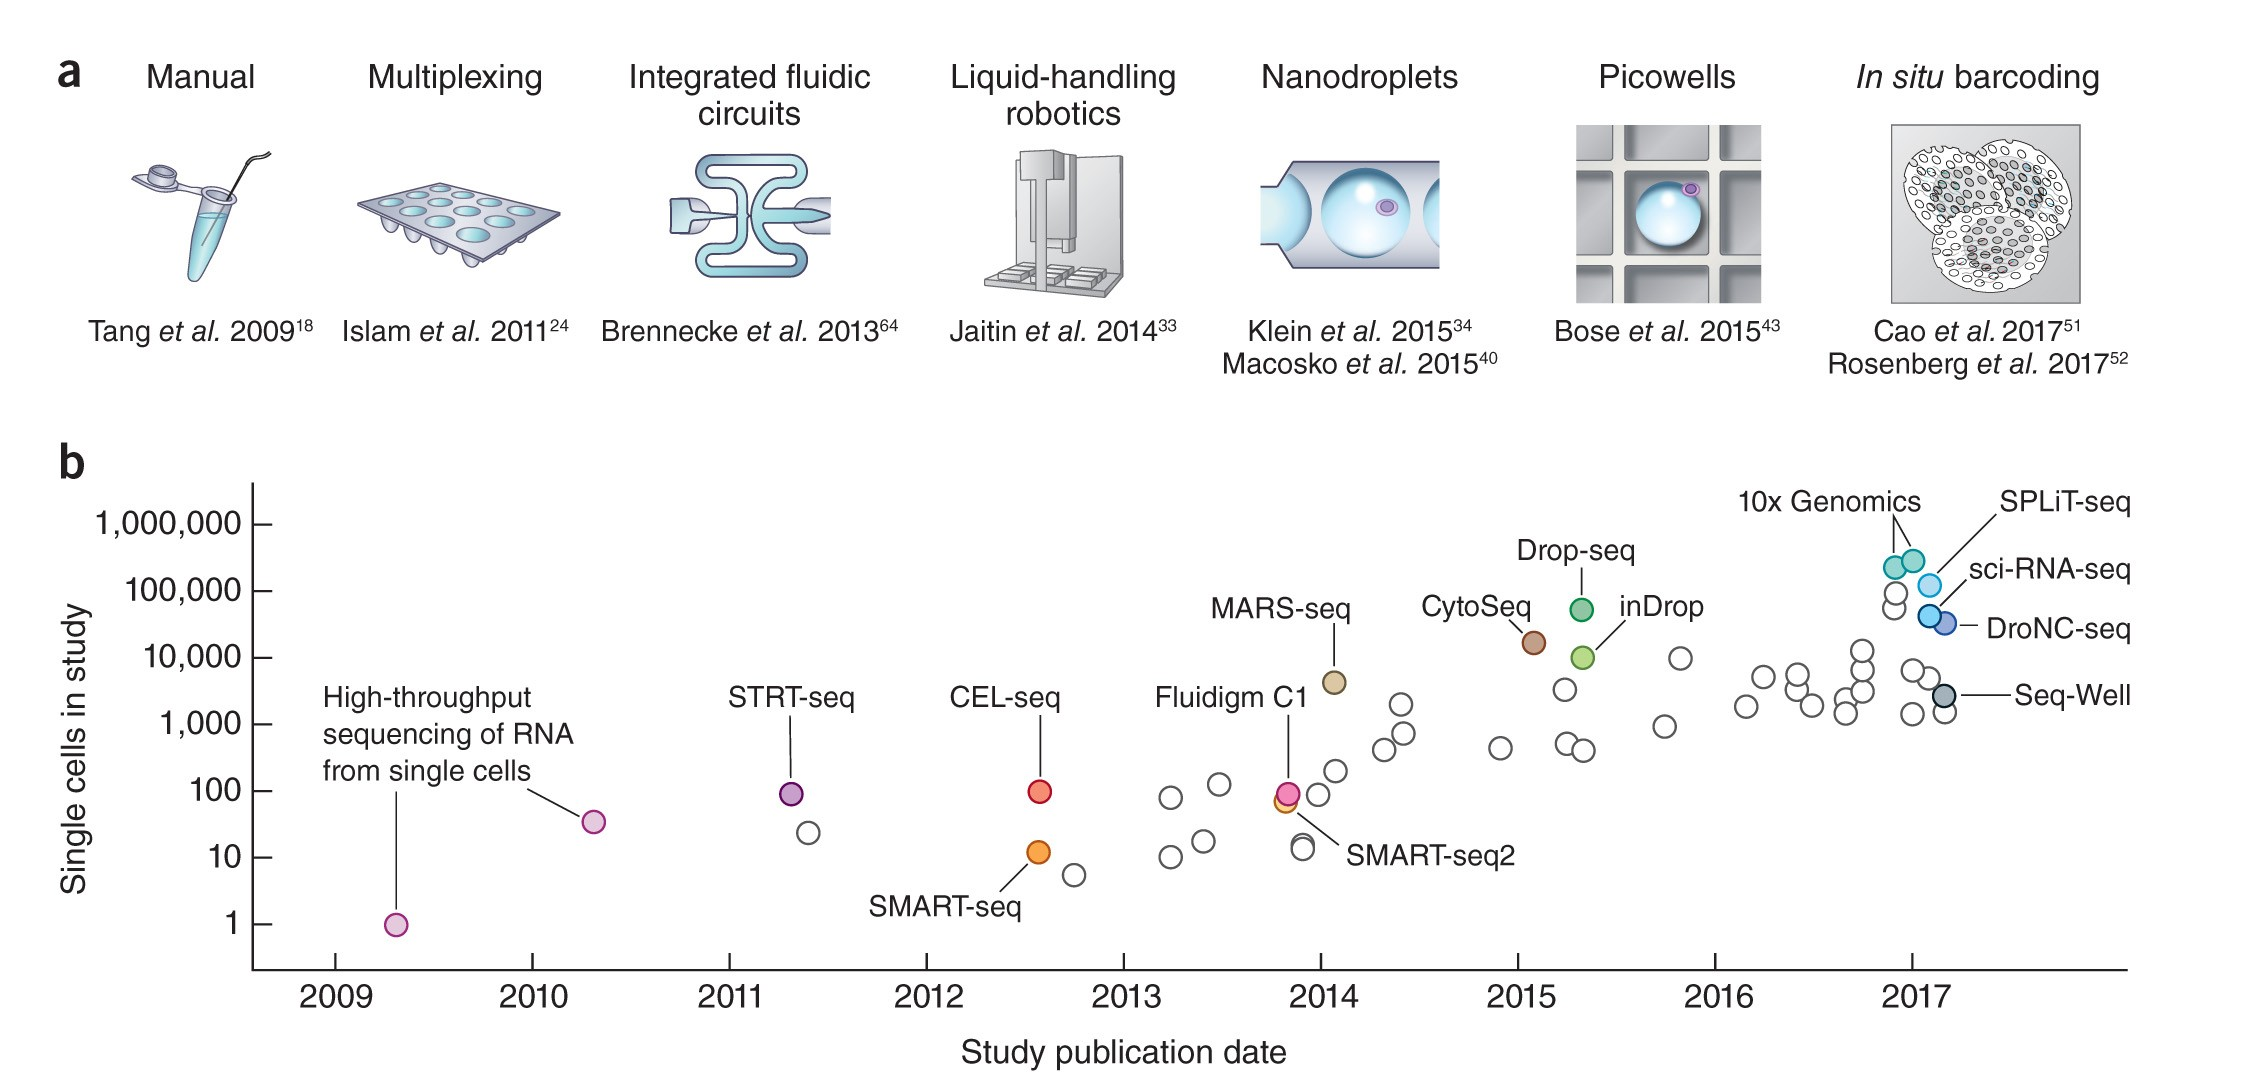
\includegraphics[width=15cm]{Chapter1/Fig/scrnaseq_technologies_svensson2018.jpg}
% \caption[\textbf{scRNA-seq technologies}]{\textbf{Scale of scRNA-seq experiments}.\\
% Technologies that have allowed....

% % make own version adding SmartSeq3 etc 

% adapted from \cite{svensson2018exponential}}
% \label{fig:scrnaseq_technologies}
% \end{figure}

% \subsubsection{Plate-based technologies}

% SmartSeq2

% \subsubsection{Droplet-based technologies}

% DropSeq, 10X Genomics

% \subsubsection{other technologies}

% multi omics aproaches (\cite{stuart2019integrative})

% spatial transcriptomics

% perturb seq

% %\subsection{Analysis of scRNA-seq data}

% \subsection{Computational modelling of scRNA-seq}

% Analysis of scRNA-seq data requires a new set of considerations, largely concerning technical signals, that were not relevant for bulk RNA-sequencing work. 
% Moreover, the resolution of this single-cell data also allows a number of more powerful analysis techniques to be applied.
% This section describes, in brief, how a typical single-cell RNA-sequencing dataset may be analysed.

% \cite{stegle2015computational}

% \subsubsection{Low-level analysis}

% reads QC 

% alignment

% mapping QC

% \subsubsection{Normalisation and batch correction}

% Count matrix
% 10 Genomics: UMI counts
% Smasrtseq2: expected counts or TPM (similar to bulk)

% cell QC (e.g. remove cells with less than xx total counts, yy total genes)
% possibly deal with doublets etc - in our case, donor assignment is also here

% normalisation (account for differences due to read coverage etc)

% log transformation (variance stabilising)

% \textbf{feature selection} (isolate most informative genes, e.g. highly variable genes - HVGs)\\

% genes that behave differently from your expected mean-variance relationship

% optional: centering+scaling - standardizing

% batch correction (stronger than normalisation) 
% mutual nearest neighbours (MNN, \cite{haghverdi2018batch}) - and then fastMNN
% canonical correlation analysis (CCA, implemented in Seurat \cite{butler2018integrating}), Stuart et al 2019
% LIGER iNMF (negative matrix factorisation),
% Harmony (\cite{nowotschin2019emergent}) - iterative soft k means (fastest)
% Welch et al 2019, Korsunsky et al 2019


% \subsubsection{Computational analysis}

% \textbf{dimensionality reduction}

% \gls{pca} was first introduced by Pearson over a hundreds years ago (\cite{}, see section 1), yet remains one of the most widely used tools \\

% \textbf{clustering}

% unsupervised\\

% \textbf{pseudotime}

% PCA, diffusion maps\\

% \textbf{DE}

% DESeq, edgeR



% \subsubsection{Visualisation techniques}

% Even after application of a dimension-reduction procedure, a typical dataset will retain more than three biologically important dimensions in its new subspace, which makes visual representation of the data challenging. 

% Transforming high-dimensional data into a human-readable format is therefore an important challenge for single-cell data interpretation.

% scRNA-seq data visualisation techniques used in this thesis: 



% \begin{itemize}
%     \item \gls{pca}
%     \item t-distributed stochastic neighbour embedding (tSNE) \cite{maaten2008visualizing}
%     \item uniform manifold approximation and projection (UMAP) \cite{mcinnes2018umap}
% \end{itemize}


% Workflow packages:

% \begin{itemize}
%     \item scanpy
%     \item scater / scran / Single cell experiment (SCE)
%     \item seurat
%     \item SINCERA
% \end{itemize}




% \subsection{General applications of scRNA-seq in biology}

% Studies of single-cell transcriptomes allow us to directly investigate properties of individual cells, i.e. mRNA abundance. 
% Thus gene regulation is analyzed at the single cell level and, unlike traditional bulk RNA- sequencing, cell-to-cell heterogeneity can be considered.

% By measuring gene expression in development, differentiation, or other responses, we can start to understand cellular phenotypes as well as the regulatory processes that determine these phenotypes. 
% In many experiments cells are sampled at many time points and gene expression is assessed.

 
% \subsubsection{Atlases}

% Human Cell Atlas (HCA)

% The human cell atlas aims to provide a comprehensive reference map of all human cells
% \cite{rozenblatt2017human}
% \subsubsection{Cancer}
% \subsubsection{Immunology}
% \subsubsection{Development}

% developmental trajectories 
% A particular advantage of single-cell methods is the ability to capture cells at various developmental
% stages in a single experiment.

% \subsubsection{lineage tracing}

\newpage

\subsection{The `resolution revolution'}
\label{sec:scrnaseq}

The first single-cell RNA sequencing (scRNA-seq) experiment was published in 2009, and the authors profiled only eight cells \cite{tang2009mrna}. 
Only 7 years later, 10X Genomics released a dataset of more than 1.3 million cells \cite{102016our}.
All in all, in the last decade, over 1,000 scRNA-seq datasets have been published 
\cite{svensson2018exponential, svensson2019curated, svensson2020single},
using a number of different technologies 
\cite{islam2011characterization, hashimshony2012cel, ramskold2012full, picelli2013smart, sasagawa2013quartz, jaitin2014massively, macosko2015highly,klein2015droplet, gierahn2017seq, zheng2017massively, hagemann2020single}
(Fig. \ref{fig:scrnaseq_technologies}).

\begin{figure}[h]
\centering
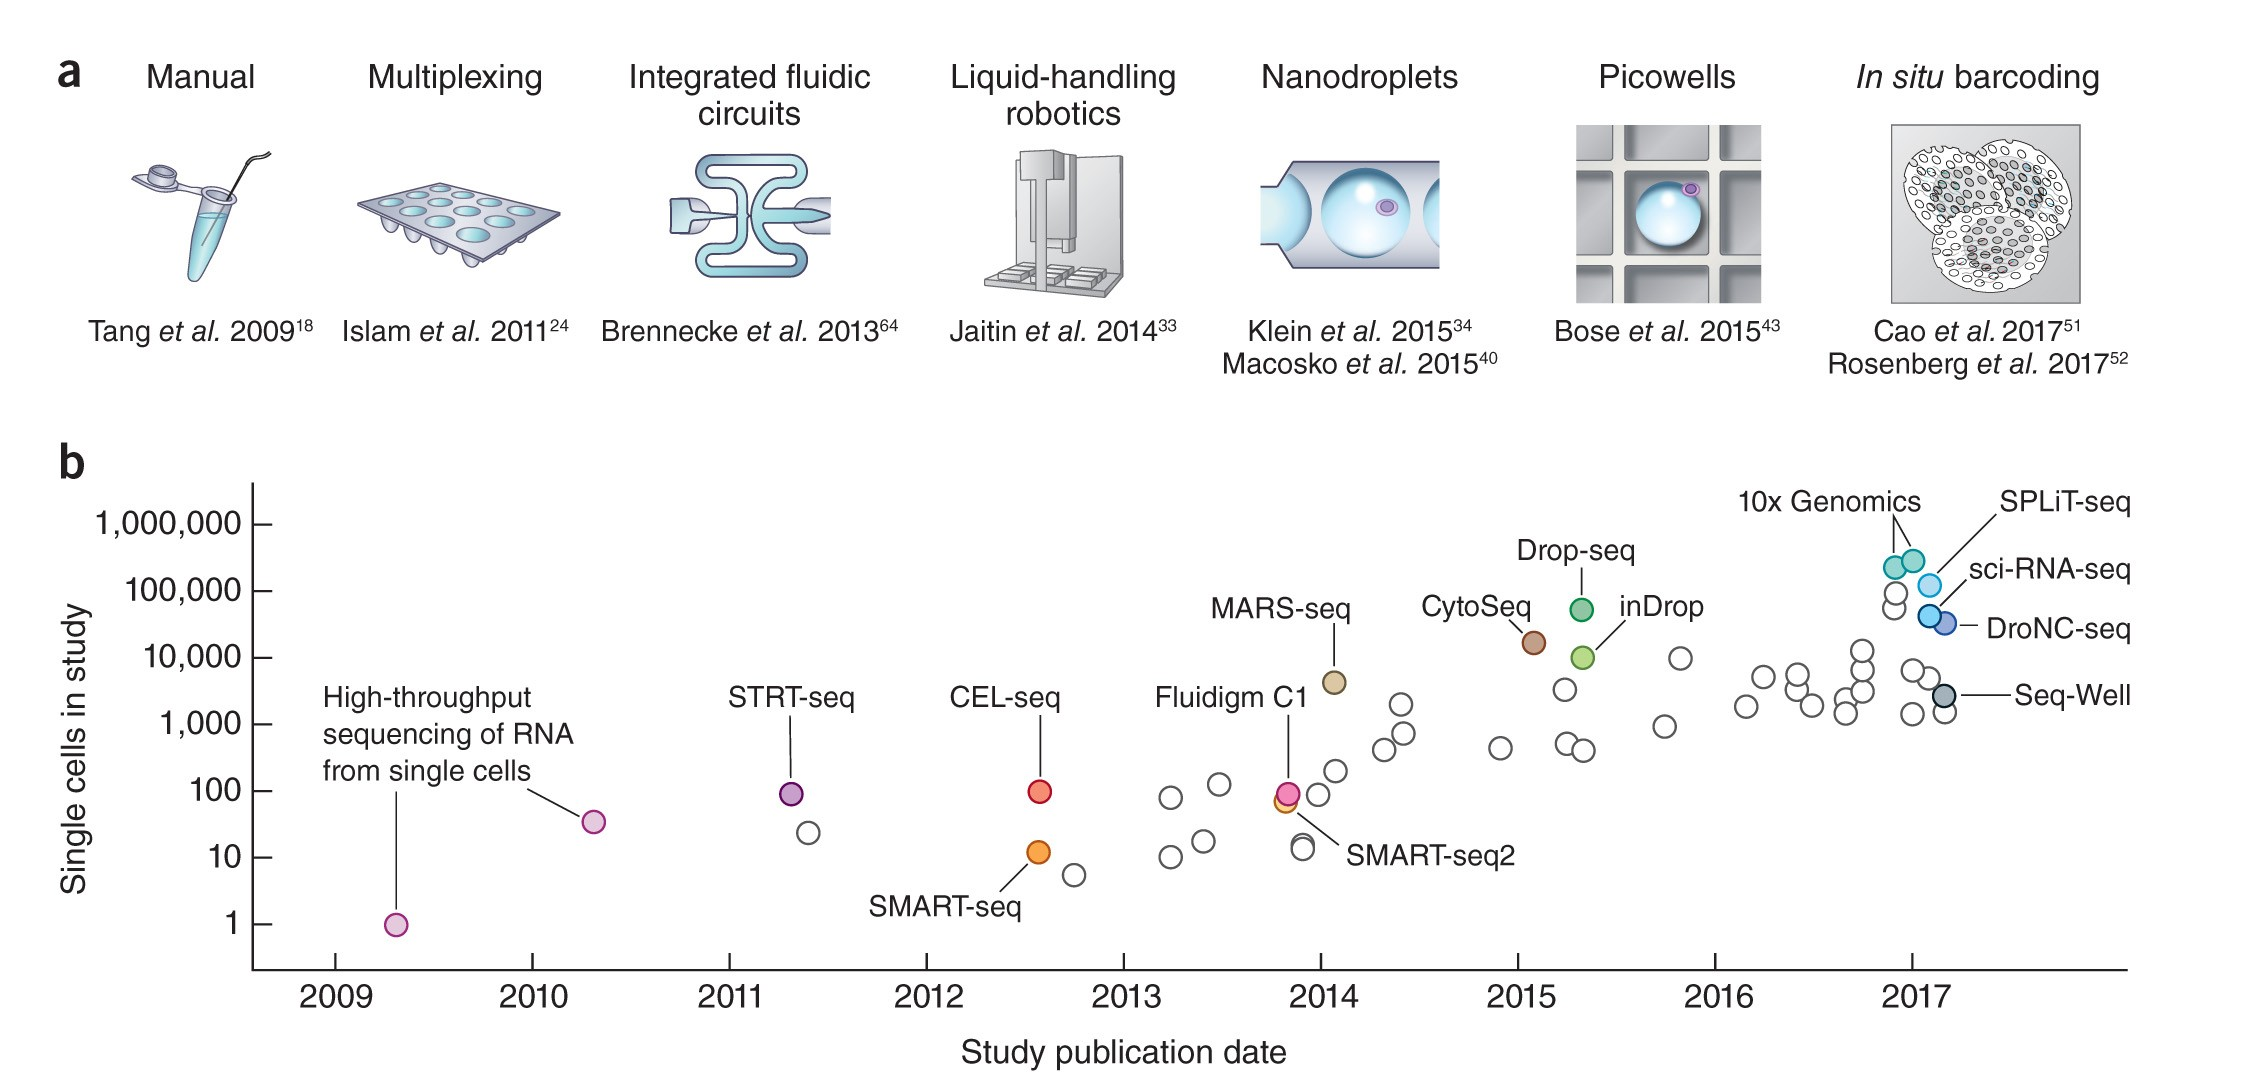
\includegraphics[width=15.5cm]{Chapter1/Fig/scrnaseq_technologies_svensson2018.jpg}
\caption[scRNA-seq technologies]{\textbf{Scale of scRNA-seq experiments}.\\
(a) Key technological advances that have allowed jumps in experimental scale, and (b) correspondingly increasing numbers of cells reported in representative publications, by publication date.
Key technologies are indicated.
% (make own version adding SmartSeq3 etc)
Adapted from \cite{svensson2018exponential}.}
\label{fig:scrnaseq_technologies}
\end{figure}

Today, scRNA-seq is an established technique, and methods are available to efficiently and reliably perform low-level analyses such as read alignment, cell calling and visualisation \cite{maaten2008visualizing, mcinnes2018umap} as well as to perform higher level tasks such as batch correction \cite{haghverdi2018batch, butler2018integrating, nowotschin2019emergent, stuart2019comprehensive, welch2019single, polanski2020bbknn}, clustering \cite{kiselev2017sc3, traag2019louvain} and pseudotime inference \cite{haghverdi2016diffusion}.\\

In some cases, those methods have been directly borrowed from bulk RNA-sequencing methods; other times, methods tailored specifically for single cell data were proposed \cite{stegle2015computational}.
A typical workflow for single cell RNA-seq data implemented in R can be found on Bioconductor\footnote{at https://bioconductor.org/packages/devel/bioc/vignettes/scran/inst/doc/scran.html and

https://osca.bioconductor.org} using scRNA-seq specific R packages scran \cite{lun2016step, risso2016scrnaseq}, scater \cite{mccarthy2017scater}, and SingleCellExperiment 
\cite{lun2019singlecellexperiment}.
Other pipelines for scRNAseq data analysis include 
Seurat \cite{butler2018integrating},
Scanpy \cite{wolf2018scanpy}, 
and SINCERA \cite{guo2015sincera}.


% Here I will only mention a few key steps.



% \subsubsection{Low-level analysis}
% reads QC 
% alignment
% mapping QC

% cell QC (e.g. remove cells with less than xx total counts, yy total genes)
% possibly deal with doublets etc - in our case, donor assignment is also here
% normalisation (account for differences due to read coverage etc)
% log transformation (variance stabilising)

% feature selection (isolate most informative genes, e.g. highly variable genes - HVGs)
% genes that behave differently from your expected mean-variance relationship



% Several platforms implement the entire processing workflow, or at least large portions of it.
% These include R packages seurat \cite{stuart2019comprehensive} and SINCERA (SINgle CEll RNA-seq profiling Analysis, \cite{guo2015sincera}) and python package scanpy \cite{wolf2018scanpy}. 



% \subsection{Computational modelling of scRNA-seq}

% Analysis of scRNA-seq data requires a new set of considerations, largely concerning technical signals, that were not relevant for bulk RNA-sequencing work. 
% Moreover, the resolution of this single-cell data also allows a number of more powerful analysis techniques to be applied.
% This section describes, in brief, how a typical single-cell RNA-sequencing dataset may be analysed.



% \subsubsection{Normalisation and batch correction}

% Count matrix
% 10 Genomics: UMI counts
% Smartseq2: expected counts or TPM (similar to bulk)



% \textbf{feature selection} (isolate most informative genes, e.g. highly variable genes - HVGs)\\

% genes that behave differently from your expected mean-variance relationship

% optional: centering+scaling - standardizing

% batch correction (stronger than normalisation) 
% mutual nearest neighbours (MNN, \cite{haghverdi2018batch}) - and then fastMNN
% canonical correlation analysis (CCA, implemented in Seurat \cite{butler2018integrating}), Stuart et al 2019
% LIGER iNMF (negative matrix factorisation),
% Harmony (\cite{nowotschin2019emergent}) - iterative soft k means (fastest)
% Welch et al 2019, Korsunsky et al 2019


% \subsubsection{Computational analysis}

% \textbf{dimensionality reduction}

% \gls{pca} was first introduced by Pearson over a hundreds years ago (\cite{}, see section 1), yet remains one of the most widely used tools \\

% \textbf{clustering}

% unsupervised\\

% \textbf{pseudotime}

% PCA, diffusion maps\\

% \textbf{DE}

% DESeq, edgeR



% \subsubsection{Visualisation techniques}

% Even after application of a dimension-reduction procedure, a typical dataset will retain more than three biologically important dimensions in its new subspace, which makes visual representation of the data challenging. 

% Transforming high-dimensional data into a human-readable format is therefore an important challenge for single-cell data interpretation.

% scRNA-seq data visualisation techniques used in this thesis: 



% \begin{itemize}
%     \item \gls{pca}
%     \item t-distributed stochastic neighbour embedding (tSNE) \cite{maaten2008visualizing}
%     \item uniform manifold approximation and projection (UMAP) \cite{mcinnes2018umap}
% \end{itemize}

\newpage

\subsection{Single cell eQTL mapping}

With the ability to identify cell types and states in an unbiased manner \cite{kolodziejczyk2015technology, trapnell2015defining}, the use of population-scale scRNA-seq data is uniquely positioned to provide an extra layer to our understanding of the genetic regulation of expression across a plethora of cell types and states, when combined with genotype information.
As a consequence, single cell eQTL mapping has emerged as a field and promises to improve our understanding of genetic regulation both in health and disease across tissues \cite{wills2013single, van2018single, kang2018multiplexed, sarkar2019discovery, cuomo2020single, jerber2020population, van2020single1}.\\

When performing eQTL mapping using scRNA-seq profiles, a first important step is to verify the feasibility of traditional `mean level' eQTL mapping, i.e. reproduce eQTL previously identified using bulk RNA-seq.
Only then can we explore new avenues and alternative types of eQTL analyses, which are especially enabled by the single cell resolution (Fig. \ref{fig:sc_eqtl}).

\begin{figure}[h]
\centering
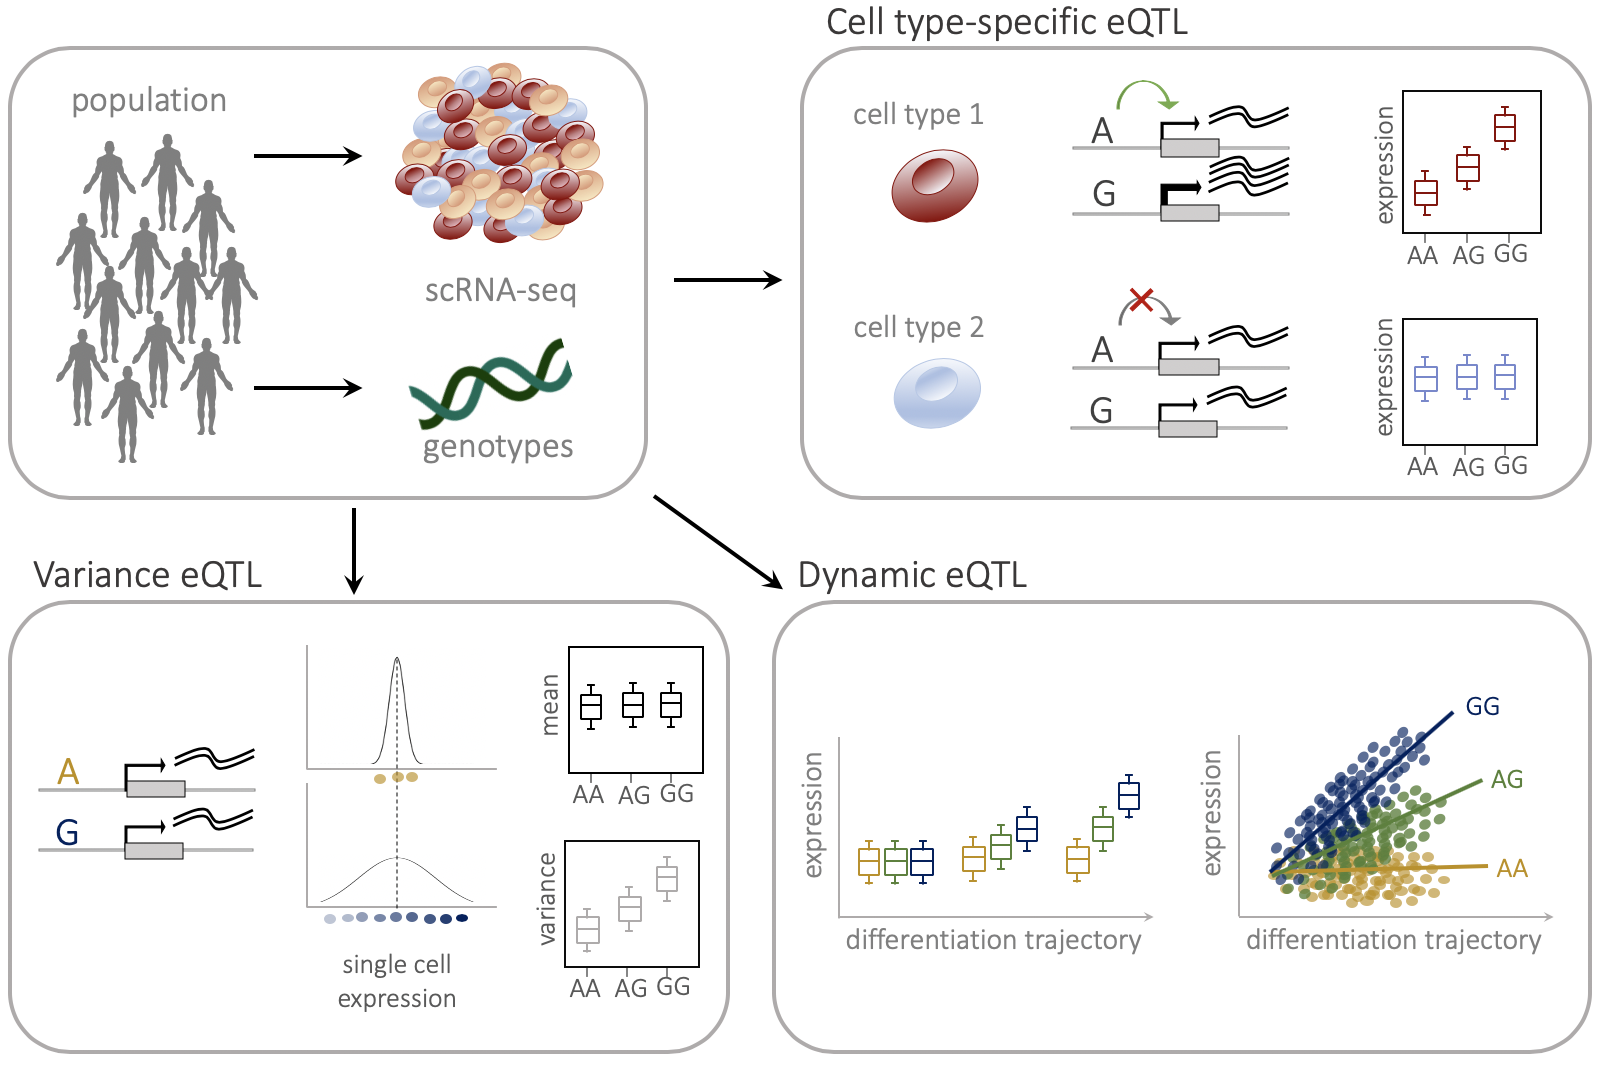
\includegraphics[width=15cm]{Chapter3/Fig/sc_eqtl.png}
\caption[Single cell eQTL]{\textbf{Overview of single cell eQTL mapping methods}.\\
(a) Setup: matched genotypes and scRNA-seq data from several individuals.
(b) Cell type-specific eQTL.
(c) Variance eQTL
(d) Dynamic/interaction eQTL.}
\label{fig:sc_eqtl}
\end{figure}

In this chapter, we address the first point (i.e. mapping mean-level sc-eQTL).
To do so, we leverage bulk and single cell gene expression of matched human \gls{ipsc} lines from around 100 donors to identify general guidelines for \gls{eqtl} mapping using scRNA-seq data.
% We compare several manners of normalising and aggregating expression across cells per donor as well as different models to test for \gls{eqtl} and compare to equivalent results obtained when using bulk RNA seq data.
% Whilst for most individuals we have plate-based sc-RNAseq data (SmartSeq2, \cite{picelli2013smart}), we also have data using the 10X Genomics platform \cite{zheng2017massively} for a subset of around 30 samples, which allows us - to an extent - to also compare results across single cell technologies.

\newpage

\section{What is different in single cell data?}

When we perform \gls{eqtl} mapping, we are interested in finding differences in expression level between individuals, when stratified by their genotypes at a genomic locus of interest. 
Under the assumption that we are looking at an otherwise homogeneous population of cells (e.g. all cells are from the same cell type), it is reasonable to consider the total (or the average) expression for each individual and gene, across all cells.
When we use bulk RNA sequencing expression profiles, that is essentially what happens: all cells from an individual are pooled, the mRNA is extracted, reverse-transcribed to cDNA, and then sequenced. 
The resulting reads are then mapped onto a reference genome, and the expression level of each gene is quantified as the number of reads (raw counts) obtained from one donor that uniquely map to that gene, after normalisation, e.g. transcripts per million (TPM)\footnote{i.e. for every 1,000,000 RNA molecules in the RNA-seq sample, x came from this gene/transcript.}. 
A bulk RNA-seq experiment, therefore, results in one individual measure of `abundance' of each gene for each donor. 
Such measure is the results of aggregating over 
hundreds of thousands of cells
% XX-YY cells (ZZ on average, \cite{})
and, at least for expressed genes (e.g. average TPM > 1), the vector of gene expression across individuals follows a distribution that can be approximated as Gaussian \cite{piras2015reduction}.
% \\
% The intuition here is that 
% Pool of RNA transcripts from many genes (low probability for a given gene), get a sample to sequence. 
% Poisson: sampling from large n, small p (samples are technical replicates)
% (biological replicates - NB > Poisson, larger variance )
% As discussed,
% % in section 1.3 of the Introduction, 
% robust experimental methods are now available to assay expression profiles of individual cells, using scRNA-seq.
% , allowing to assay the genome-wide transcriptome of hundreds to thousands of individual cells. 
On the other hand,
whilst scRNA-seq data provides increased resolution and promises great insights into cellular function, the data also are much sparser, and the amount of cells that can be assayed for an individual is limited compared to bulk (often as little as 10-100 cells per individual). 
In addition, the number of cells that can be assessed often varies substantially from individual to individual.
As a result, the distribution of total counts from a single cell experiment as opposed to its corresponding bulk experiment is shifted downwards (lower mean) and more spread out (higher variance, Fig. \ref{fig:sc_bulk_counts}).
% (on average XX compared to YY for bulk RNA-seq, \cite{}).
% Moreover, in addition to observing a smaller number of cells (and therefore total reads) for an individual as compared to bulk, the read distribution typically does not follow a normal distribution, mostly due to very different amounts of reads coming from different donors. \\

\begin{figure}[h]
\centering
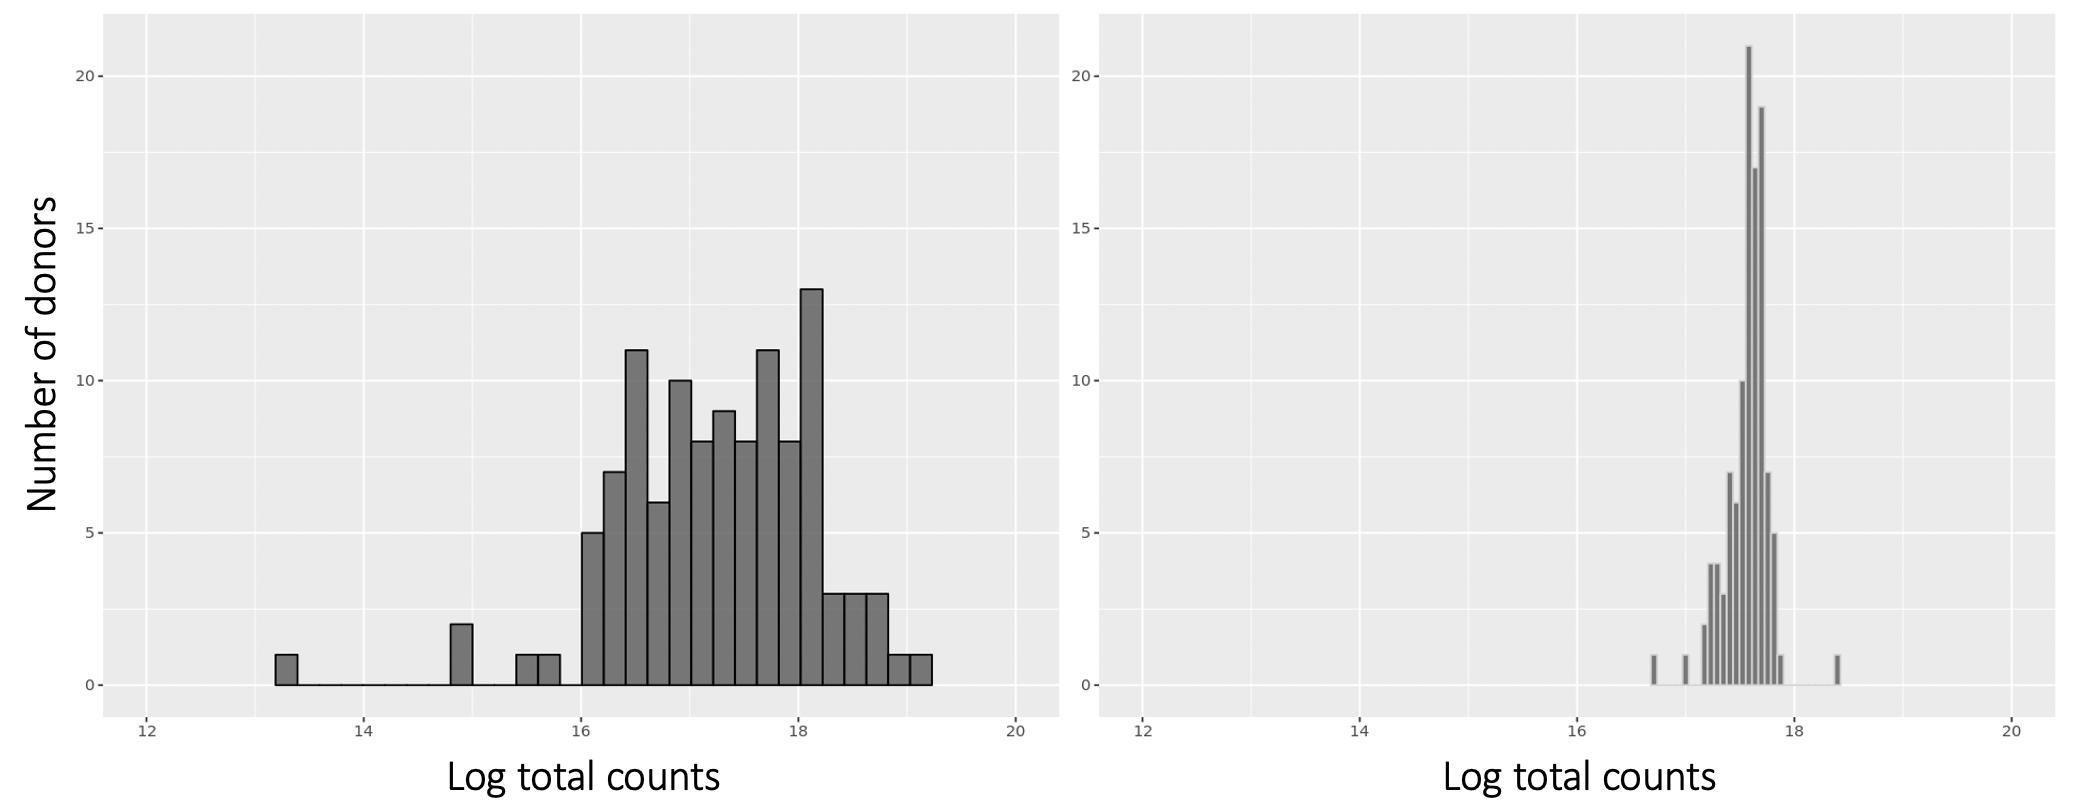
\includegraphics[width=13cm]{Chapter3/Fig/count_distribution_sc_vs_bulk.png}
\caption[Distribution of reads]{\textbf{Distribution of reads}.\\
Distribution of total reads per individual for matched iPSC data (109 individuals) using single cell (left, from \cite{cuomo2020single}) and bulk (right, from \cite{mirauta2018population}) RNA-seq data.}
\label{fig:sc_bulk_counts}
\end{figure}
% This is in part due to the `double sampling' that is inherent of the technology: there is a chance of not sampling any reads from one gene in one cell, and there is a chance of not sequencing any reads from that cell at all.

% Add differences in number of total reads, read distribution, describe “double sampling” process.

\newpage

\section{Data}

The data I use here to benchmark methods for single cell eQTL mapping was generated by colleagues at the Sanger Institute\footnote{The Ludovic Vallier lab, at the Wellcome Trust Sanger Institute, Cambridge, UK.
Full acknowledgment and contributions for this project can be found in the next chapter, at page \pageref{contr:chapter4}.}, using human iPSC lines from the \gls{hipsci} resource (see section \ref{sec:ips_genetics}). 
They were generated as part of a larger study, where iPSC lines from over 100 donors are differentiated towards definitive endoderm.
Cells were collected at four time points (day0, day1, day2, day3) and sequenced using Smartseq2, a plate-based single cell technology \cite{picelli2013smart}.
This study was published early this year \cite{cuomo2020single}, and I discuss the key results from it in the next chapter (Chapter 4).\\

% In this chapter, 
Here,
I focus on the earliest time point (i.e. day0), where cells are still pluripotent, prior to cell differentiation.
After QC\footnote{Some QC steps were performed for all time points jointly, therefore I refer the reader to the detailed QC pipeline described in the next chapter, at page \pageref{fig:endodiff_qc_workflow}.}, we have data from 9,661 iPS cells and 11,231 genes, from 112 unique unrelated donors, across 24 differentiation experiments. 
% We expect iPS cells to be fairly homogeneous, so it is the perfect cell type to perform this kind of study. 
% \\
% Add QC steps here? Maybe briefly and then refer to chapter 4.
% Also more on HipSci lines (used): sex, age, ethnicity
% \subsection{Comparison partners}
Additionally, we have matched deep bulk RNA-sequencing profiles generated as part of the HipSci project \cite{kilpinen2017common}, for the vast majority of cell lines used (109/112, 97\%).
% , as well as for a large number of other HipSci lines (676 human iPSC lines from 462 unique donors in total).
Finally, we have scRNA-seq data measured using a droplet-based technology (10X Genomics \cite{zheng2017massively}) for a subset of common samples (29 iPSC lines, from five experimental batches). 

\begin{figure}[h]
\centering
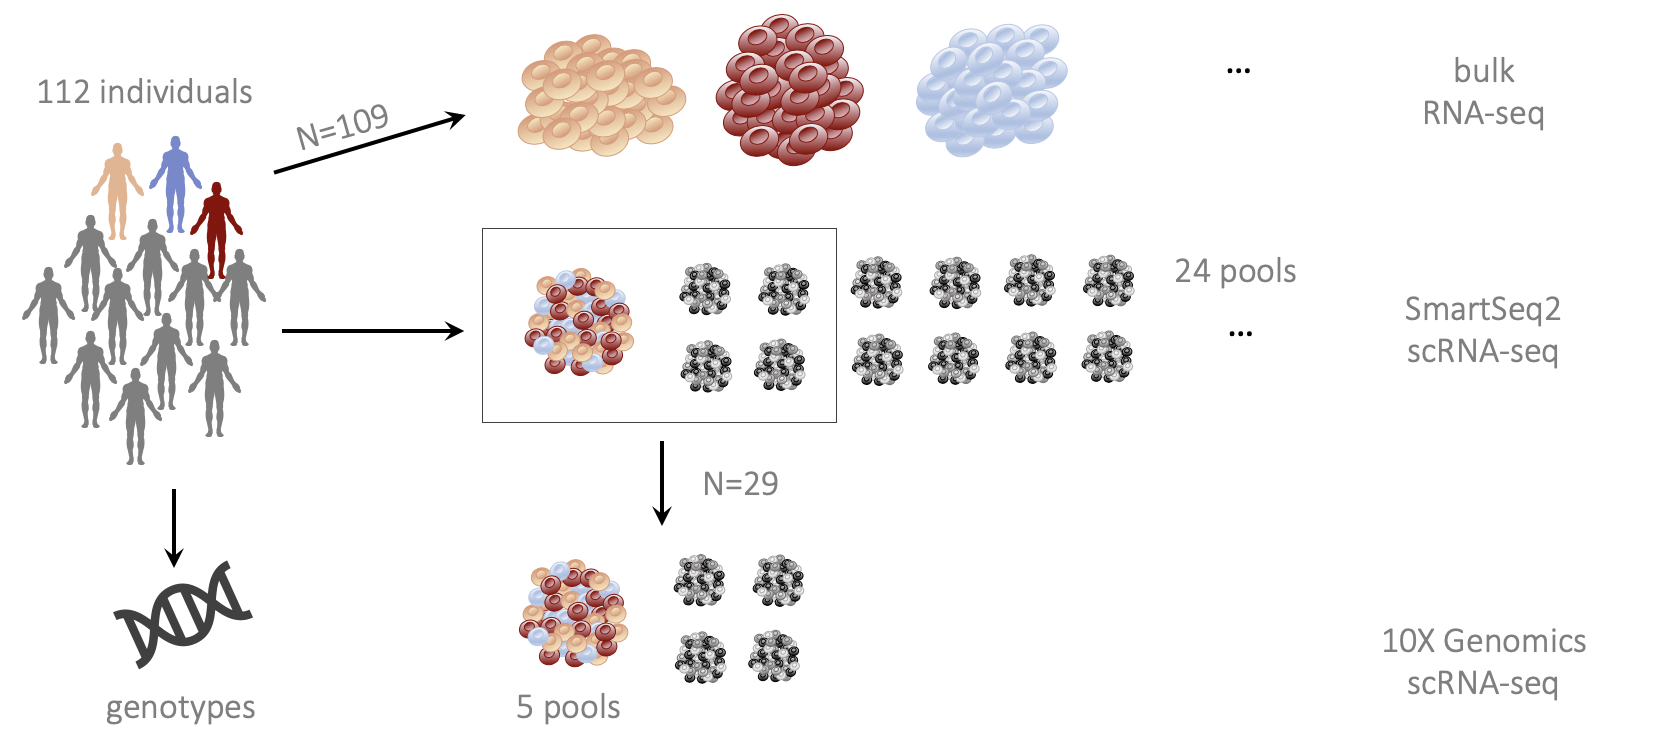
\includegraphics[width=14.5cm]{Chapter3/Fig/ips_data.png}
\caption[iPSC data]{\textbf{Overview of iPSC data used in this chapter}.\\
We use SmartSeq2 \cite{purcell2007plink} data from 112 iPSC lines (from 112 individuals) from \cite{cuomo2020single}, across 24 experimental pools, each containing cells from 4-6 lines (middle).
For 109 of those lines, we have bulk RNA-seq profiles from \cite{mirauta2018population}(top).
Finally, for five of the pools (corresponding to 29 individuals/lines), we also have scRNA-seq data sequenced using the 10X Genomics pipeline \cite{zheng2017massively}(bottom).}
\label{fig:ipsc_data}
\end{figure}

% \begin{itemize}
%     \item bulk RNA-seq with matched samples (i.e. individuals for which we have both bulk and sc-RNAseq data, N = 109/112)
%     \item bulk RNA-seq all samples (i.e. all samples for which we have bulk RNA-seq data, N = 462)
%     \item matched 10x scRNA-seq (for a subset of common samples, N = 29/112)
% \end{itemize}

\newpage

\section{Methods}

To map eQTL, I use a flexible pipeline written by Marc Jan Bonder, to which Bogdan Mirauta, Daniel Seaton, Na Cai and myself have also contributed. 
It is a wrapper around LIMIX \cite{lippert2014limix, casale2015efficient}, and it is publicly available at \url{https://github.com/single-cell-genetics/limix_qtl}. \\

Here, I performed \textit{cis} eQTL mapping, considering all common variants (minor allele frequency >5\%) within a \textit{cis}-region spanning 250 kb up- and downstream of the gene body for \textit{cis} QTL analysis. 
For each gene-SNP pair, the association test was performed using a linear mixed model (LMM):

\begin{equation}
    \mathbf{y} = \sum_i^{10}\alpha_i \mathbf{PC}_i + \mathbf{g}\beta + \mathbf{u} + \boldsymbol{\psi},  
\end{equation}
where 
\begin{itemize}
    \item $\mathbf{y}$ is the $N \times 1$ standardised\footnote{Centered at 0 and scaled to have variance = 1.} expression phenotype vector,
    \item we included the first 10 principal components calculated on the expression values in the model as linear covariates\footnote{This is a common approach to correct for possible batch effects, which usually affect the expression of many genes, and therefore are detectable in the principal components of expression. 
    Moreover, these global effects are orthogonal to the effects of a single variant on the expression of one gene.}, and learn the corresponding weights $\alpha_i$,
    \item $\mathbf{g}$ is the $N \times 1$ vector of alleles for each sample at the locus tested (modelled as the number of minor alleles present - 0, 1 or 2), and $\beta$ is the corresponding effect size,
    \item $\mathbf{u} \sim \mathcal{N}(\mathbf{0}, \sigma_g^2\mathbf{K})$, where $\mathbf{K}$ is a $N \times N$ kinship matrix estimated using PLINK \cite{purcell2007plink},
    \item and $\boldsymbol{\psi} \sim \mathcal{N}(\mathbf{0}, \sigma_n^2\mathbf{I})$, where $\mathbf{I}$ is the $N \times N$ identity matrix.\\
\end{itemize}

% Association tests were performed using a linear mixed model (LMM), accounting for population structure and sample repeat structure (see below) as random effects (using a kinship matrix estimated using PLINK\cite{purcell2007plink}).
% , with no observed confounding between population structure and experimental batch (Supplementary Fig. 24). 
All models were fitted using LIMIX \cite{lippert2014limix, casale2015efficient}. 
The significance was tested using a likelihood ratio test (LRT) (i.e. $\beta \neq 0$, see section \ref{eq:Linear_regression_genetics}).
In order to adjust for multiple testing, we used an approximate permutation scheme, analogous to the approach proposed in Ongen \textit{et al}. \cite{ongen2016fast}. 
Briefly, for each gene, we generated 1,000 permutations of the genotypes while keeping covariates, kinship, and expression values fixed. 
We then adjusted for multiple testing using this empirical null distribution. 
To control for multiple testing across genes, we then applied the Storey procedure \cite{storey2003statistical}. 
Genes with significant eQTL were reported at FDR < 10\%.

\newpage

\section{Single cell eQTL map of iPS cells}

First, we tested for associations between common genetic variants and gene expression in \glspl{ipsc} using our SmartSeq2 single cell data.\\

To reproduce bulk-like abundance measurements, we considered a gene's average expression level (measured as log2(CPM+1)\footnote{CPM: counts per million, mapped reads are counts-scaled by the total number of fragments sequenced, times one million.}) for each sample, across cells.
Since we did not use any batch correction method on the single cell expression data \textit{a priori}, we cannot exclude differences across batches.
As internal control we have, for a subset of donors (23/112), data from two (or three, in one case) distinct experimental batches.
We therefore compute average expression levels not for each individual, but for each individual-experiment combination (i.e. individualA-experiment1, individualA-experiment2), which allows to effectively correct for batch-to-batch differences using PCs as covariates.\\

% However, to be able to correct for possible batch differences, we considered two different average expression measures, when the same line was assessed in two different experimental batches - individual 1 in experiment A and individual 1 in experiment B are considered as two distinct samples.

% \subsection{Technical considerations}

As a result, we have in some cases replicate measures from the same individual.
% Meaning that both the genotype vector $\mathbf{g}$ and the kinship matrix $\mathbf{K}$ need to be adjusted.
This is when LMMs are especially useful, by incorporating the
Here you see why LMMs are useful, the kinship account at once for population structure and repeatedness.

\begin{figure}[h]
\centering
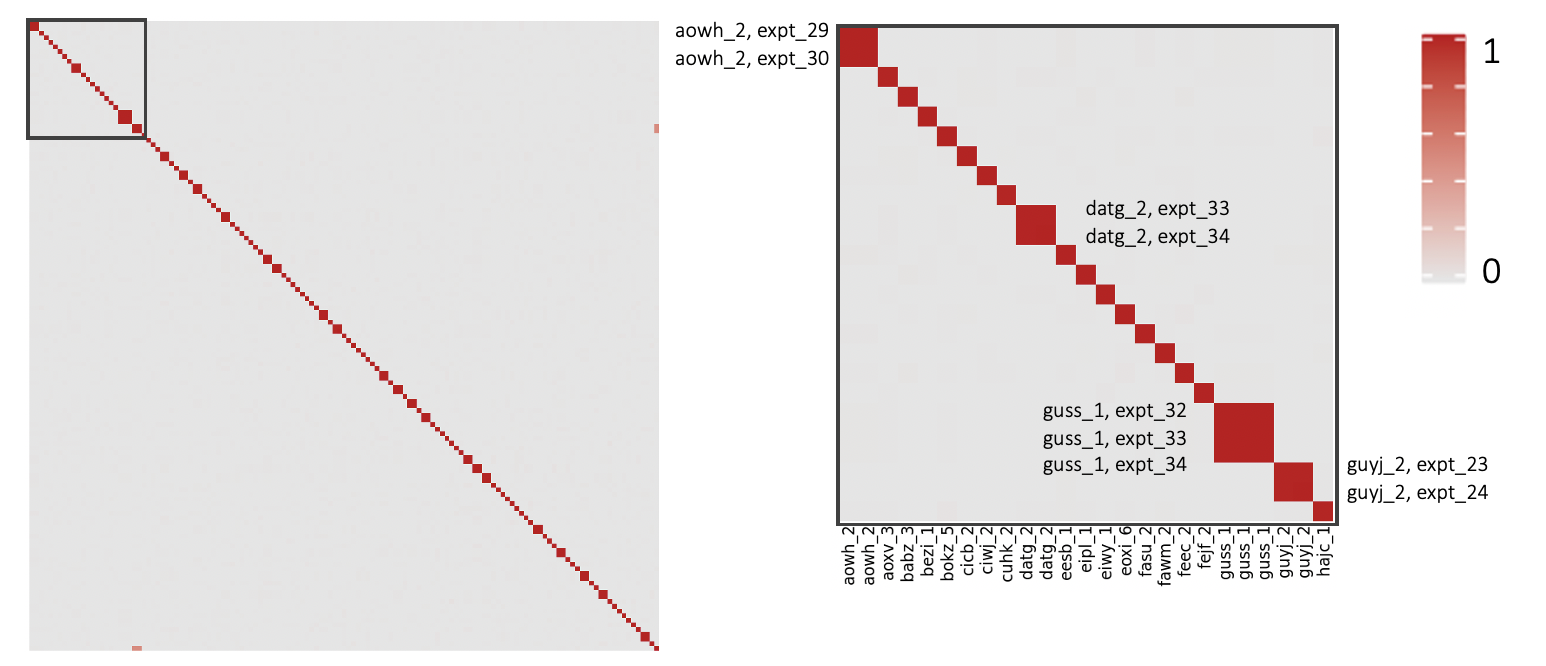
\includegraphics[width=15cm]{Chapter3/Fig/kinship_repeatedness.png}
\caption[Kinship for repeats]{\textbf{Expanded kinship highlighting repeated structure of samples used (draft}.\\
Essentially unrelated individuals, 
First 20 iPSC lines, highlighting the repeated structure.}
\label{fig:kinship_repeats}
\end{figure}

% \subsection{Results}

% CPM = readsMappedToGene * 1/totalNumReads * 10$^6$, totalNumReads - total number of mapped reads of a sample, readsMappedToGene - number of reads mapped to a selected gene

Using this approach, we identified 1,833 genes with at least one \gls{eqtl} (eGenes), at FDR <10\%, out of 10,840 genes tested (17\%). 


% \subsection{LMM}
% Association tests were performed using a linear mixed model (LMM), accounting for population structure and sample repeat structure (see below) as random effects (using a kinship matrix estimated using PLINK\cite{purcell2007plink}).
% % , with no observed confounding between population structure and experimental batch (Supplementary Fig. 24). 


\newpage

\section{Replication in bulk}

For comparison, we performed \textit{cis}-eQTL mapping using the matched bulk RNA-seq data, 
% considering only the cell lines that had been used to map iPSC eQTL from the scRNA-seq data (bulk data was available for 108 donors out of the 112 day0 single cell donors), 
and tested the same set of genes. 
This yielded 2,908 significant genes at an FDR of 10\% (out of 10,736 genes tested, 27\%). \\

Over 70\% of eQTL identified using scRNA-seq data were replicated in the bulk study, where to define replication we assessed the nominal significance (p value < 0.05) as well as the consistent direction of effect of single-cell eQTL lead variants (top variant per gene) in the full set of results from the bulk eQTL analysis (Fig. \ref{fig:sc_bulk_egenes}). \\

On the other hand, only around 50\% of the eQTL identified using bulk RNA-seq could be replicated
% \footnote{Defined as above: nominal significance (p value < 0.05) and same direction of effect.} 
in our single cell eQTL map.
However, when we subsetted to eQTL identified with bulk at a more stringent FDR threshold (1\%), the replication proportion was much larger (76\%), and the more stringent the FDR threshold, the more bulk eQTL we could replicate using single cell data (Fig. \ref{fig:sc_bulk_egenes}).
This result suggests that we are able to detect the stronger eQTL signals, but lack the power (compared to bulk) to identify smaller effects.\\

\begin{figure}[h]
\centering
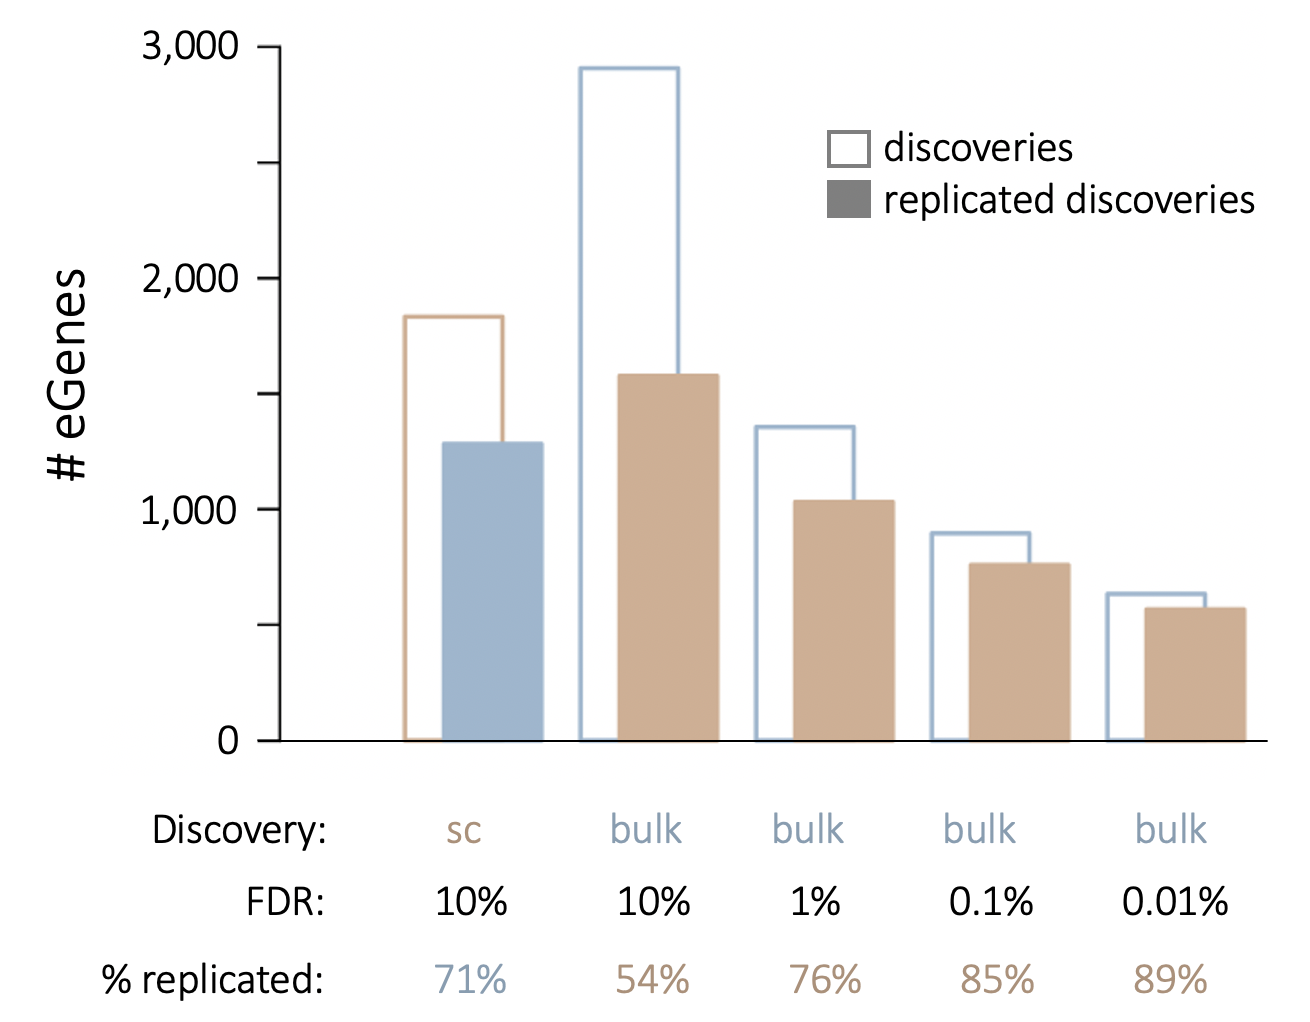
\includegraphics[width=10.5cm]{Chapter3/Fig/sc_vs_bulk_eqtl.png}
\caption[iPSC eQTL (bulk vs sc)]{\textbf{Replication of iPSC bulk eQTL using single cell data and vice versa}.\\
Replication of iPSC eQTL discovered with matched-sample bulk RNA-seq data, using single cell RNA-seq data, and vice versa.
The total number of eGenes discovered is shown, along with the number of discoveries replicated in the other dataset, at various FDR thresholds. 
% Replication of bulk eQTL in single-cell RNA-seq (SmartSeq2, here SS2) on same set of samples increases with significance ($\sim$55\% at FDR 10\%, $\sim$90\% at FDR 0.01\%, 4/112 samples were not present in the bulk RNA sequencing dataset).
sc: single cell.}
\label{fig:sc_bulk_egenes}
\end{figure}

% To compare the iPSC eQTL maps derived from bulk and single-cell RNA-seq data, we assessed the nominal significance (p value < 0.05) as well as the consistent direction of effect of single-cell iPSC eQTL lead variants (top variant per gene) in the full set of results from the bulk iPSC eQTL analysis and vice versa.

% To validate our approach, we also performed \gls{eqtl} mapping using deep bulk RNA-sequencing profiles from the same set of \gls{ipsc} lines (“iPSC bulk”; 10,736 genes tested) generated as part of the \gls{hipsci} project \cite{kilpinen2017common}, yielding consistent \gls{eqtl} ($\sim$70\% replication of lead \gls{eqtl} effects; nominal p value < 0.05).\\ 

\newpage

\section{Replication in 10x}

To further confirm our iPSC eQTL map, we performed eQTL analysis using scRNA-seq data generated from a subset of 5 experiments (29 lines) using a droplet-based approach (10x Genomics \cite{zheng2017massively}).\\

Similar to before, we assessed how many bulk-identified iPSC eQTL could be replicated using 10x samples.
Since this study is fairly underpowered with only 29 samples, we did not consider the opposite analysis, i.e. 10x discoveries replicated in bulk.
We did, however, compare results to an iPSC eQTL map using the SmartSeq2 data, when sub-setted to the same 5 experiments (and 29 lines). \\

Overall, we observe that replication of bulk eQTL using scRNA-seq is reduced when we reduce sample size (41\% compared to 54\% at FDR 10\%, 77\% compared to 89\% at FDR 0.01\%), but comparable across technologies (SmartSeq2, 10x Genomics), with SmartSeq2 slightly outperforming 10x (Fig. \ref{fig:sc_bulk_10x_egenes}).\\

\begin{figure}[h]
% \centering
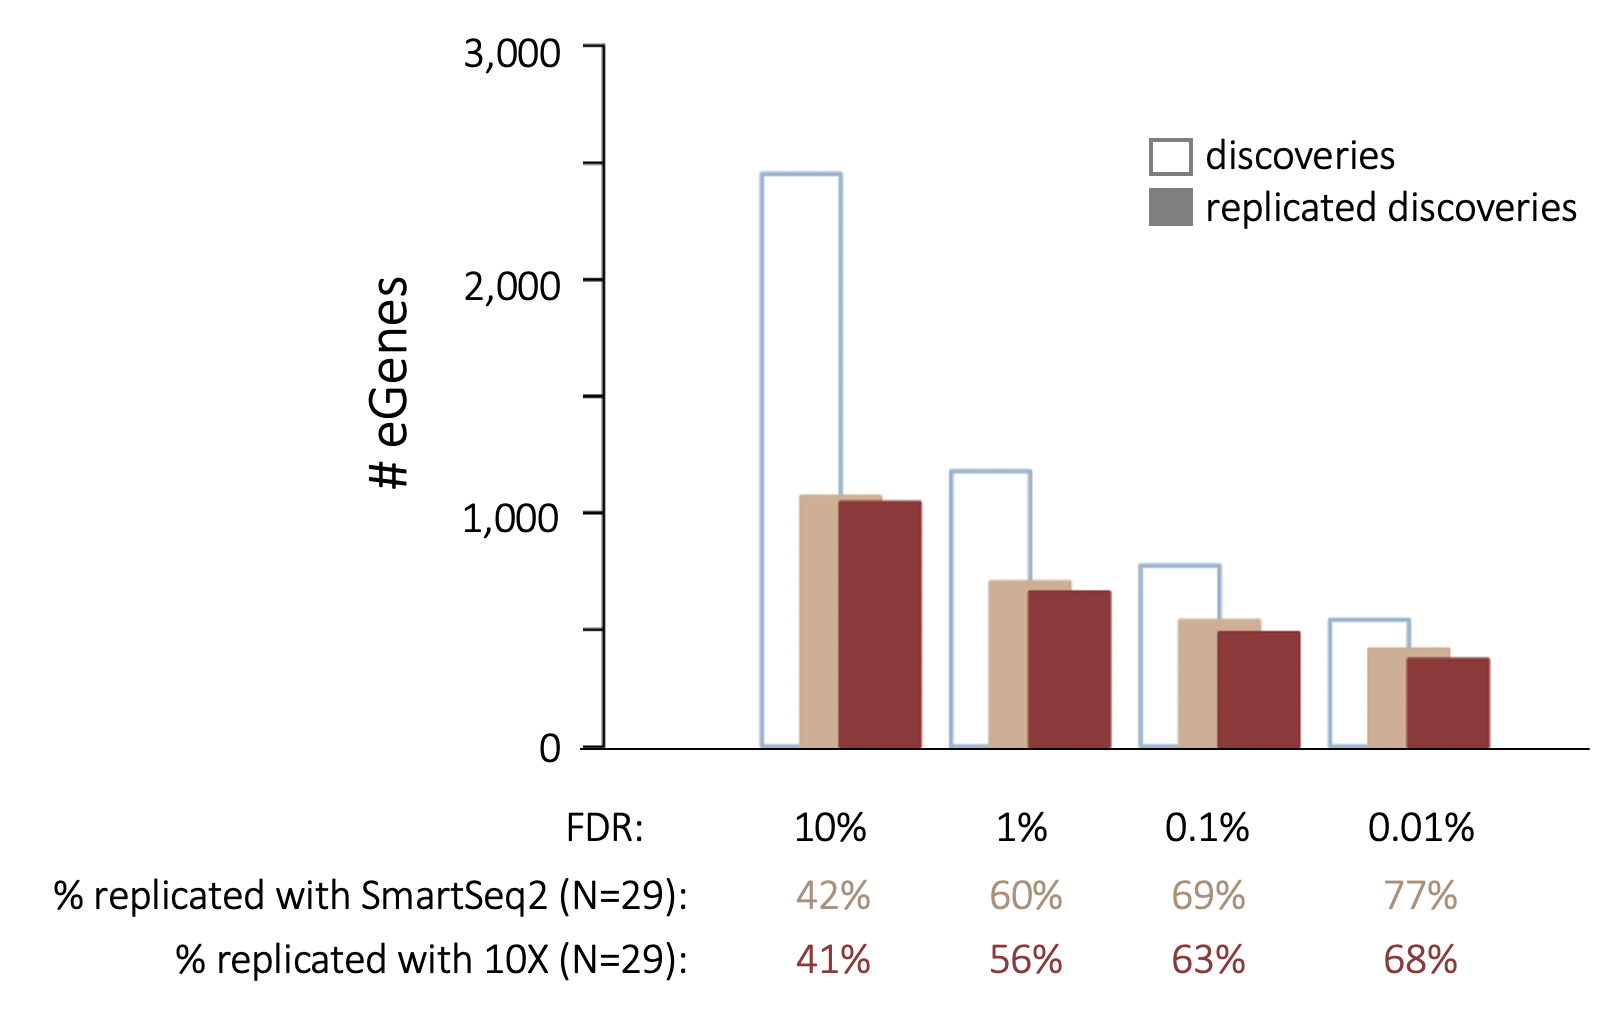
\includegraphics[width=13cm]{Chapter3/Fig/sc_vs_bulk_vs_10x.png}
\caption[iPSC bulk eQTL replication]{\textbf{Replication of iPSC bulk eQTL using single cell across technologies}.\\
Replication of iPSC eQTL discovered with bulk RNA-seq (108 samples), using single cell RNA-seq data (SmartSeq2 in sand, 10x Genomics in red). 
The total number of bulk eGenes discovered is shown, along with the number of discoveries replicated using single cell profiles, at different FDR thresholds. 
As before, replication was defined as nominal significance, at p value < 0.05, and same direction of effect. 
The same 29 samples are considered for both technologies.}
\label{fig:sc_bulk_10x_egenes}
\end{figure}

\newpage

Additionally, we found very good agreement in terms of effect size between the eQTL maps obtained using the two different single cell technologies, highlighting the robustness of the approach (Fig. \ref{fig:sc_eqtl_technologies}).\\

\begin{figure}[h]
\centering
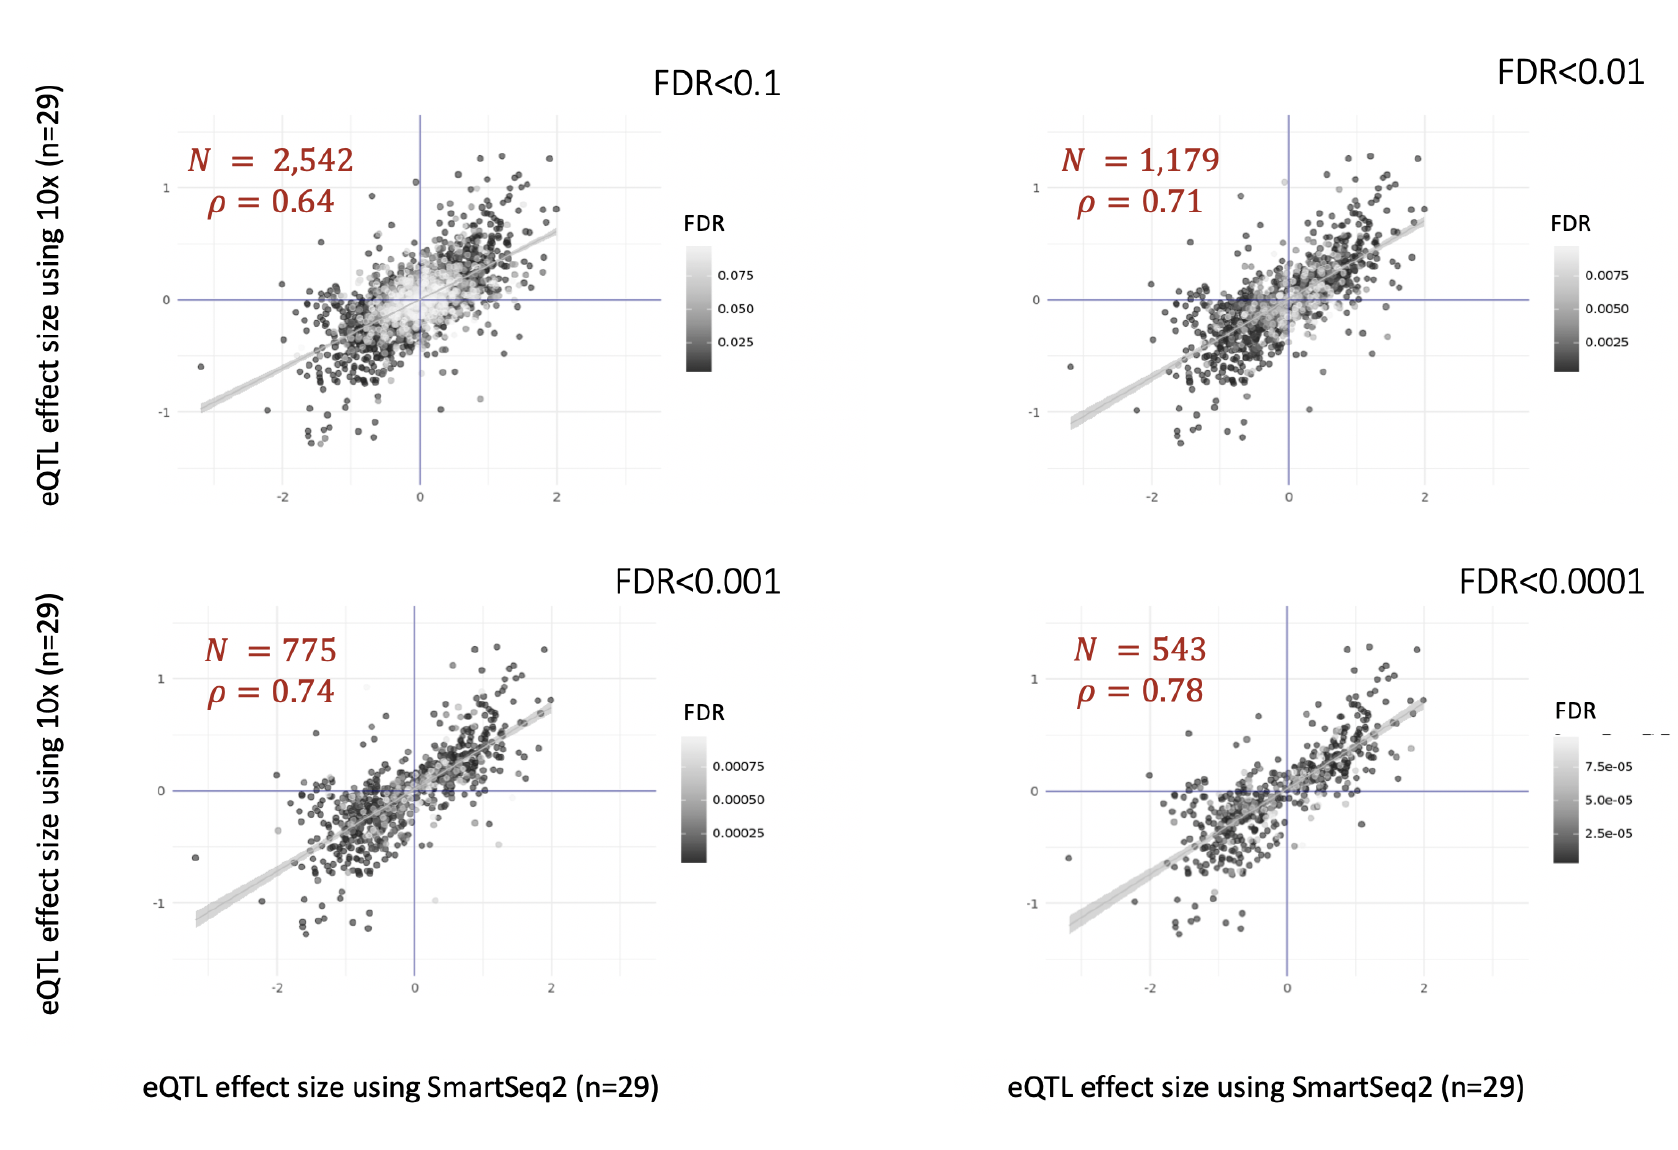
\includegraphics[width=15cm]{Chapter3/Fig/beta_comparison_ss2_vs_10x.png}
\caption[iPSC sc-eQTL replication across technologies]{\textbf{Effect size agreement between single cell technologies.}.\\
Scatterplots of eQTL effect sizes obtained when testing association of iPSC eQTL discovered using bulk RNA-sequencing (108 cell lines) using SmartSeq2 (x axis) and 10x Genomics (y axis) on cells from 5 experimental batches (experiments 31, 40, 41, 43, 44; 29 cell lines in total). 
The number of eQTL examined and the correlation between effect sizes is indicated when we consider bulk iPSC eQTL discoveries at four different FDR thresholds (0.1, 0.01, 0.001, 0.0001).}
\label{fig:sc_eqtl_technologies}
\end{figure}

As we acknowledge that the vast majority of scRNA-seq datasets presented recently use droplet-based (rather than plate-based) technology, as it allows to assess a much larger number of cells in a single experiment, it is important to show that this approach would work for such datasets as well. 
Whilst in this case we had data from too few individuals to make a very strong argument, the good concordance of results between 10x and SmartSeq2 clearly indicates that this approach should work well for all single cell RNA-seq datasets.

\clearpage

% \section{Preliminary comparison}

% The results presented so far are included in Cuomo \textit{et al}. \cite{cuomo2020single}, which I discuss in detail in the next chapter (Chapter 4). \\

% More recently, in collaboration with Marc Jan Bonder and Giordano Alvari from the Stegle group, we have worked on a best practice pipeline which extends on the work presented so far, by testing the effect of different parameters of the model, to optimise yield.
% In particular, we tested various aggregation strategies to obtain `pseudo-bulk' expression levels to use as phenotypes in the model.
% Next, we varied the type and number of `global expression effect' covariated to include in the model.
% Finally, we evaluated normalisation strategies for the expression profiles.

% % \section{Methods}

% % In order to produce bulk-like results, two main approaches can be used.

% % Under the assumption that we are looking at a single cell type, we can i) aggregate counts across all cells from an individual (e.g. taking the average expression value) and generate a `pseudo-bulk' measure, and then run the test exactly as if it were bulk; or ii) use full single cell expression, without aggregating.

% % % In this chapter, we introduce the two datasets that we will use throughout the thesis, setting the scene for all other chapters. 
% % % These are among the very first datasets of their kind, assessing single cell gene expression profiles for hundreds of genetically diverse individuals, allowing to interrogate the effect of common genetic variation on transcriptional variability.
% % % Previously, most \gls{eqtl} mapping studies in humans were performed using bulk RNA-sequencing, and most scRNA-seq studies were performed in a handful of individuals only, or in model organisms (often also limited to a few strains).
% % % Notably, one study performed \gls{eqtl} mapping using scRNA-seq \cite{van2018single} recently in blood cells. 
% % % However, this data is limited to 45 individuals and to a single time point, lacking the differentiation axis of our studies.

% % % \subsection{Datasets}

% % % \begin{itemize}
% % %     \item iPS data
% % %     \item simulated data
% % % \end{itemize}

% % \subsection{Data}

% % We use iPS data from \cite{cuomo2020single} - day0 only, etc

% % Smartseq2 \cite{picelli2013smart} data from 10,000 (get exact number) cells from 112 unique unrelated donors, across YY differentiation experiments. 

% \subsection{Aggregation strategies}

% Pseudobulk approach.
% To comprehensively investigate which aggregation method would result in most power to to identify single cell eQTL, we tried:

% \begin{itemize}
%     \item Mean: average expression across cells from each donor and sequencing run
%     \item Median: median expression across cells from each donor and sequencing run
%     \item Sum: summed expression across cells from each donor and sequencing run
%     \item Total mean: average expression across all cells from each donor, aggregated across sequencing runs
%     \item Total sum: similar to the total mean, but summing reads instead
% \end{itemize}

% Aggregation is done not only at the donor level but also for each individual sequencing run (i.e. all iPS cells from a given donor in a single sequencing run) in the mean, median and sum.
% This is done in an attempt to account for batch effects (needs explaining).
% For what we call `total' sum and mean, on the other hand, aggregation (i.e. sum or mean) is done per donor only, to maximise numbers of cells per donor.\\

% Normalisation of the scRNA-seq data was performed in two different ways depending on the aggregation method used.
% For mean and median aggregation of expression data, we first performed standard single cell data normalisation using scran/scater normalisation.
% Briefly, log2(cpm+1) using size factors..
% The mean and the median were calculated on the resulting normalised counts (Fig. \ref{fig:sc_qtl_workflow}).

% On the other hand, summed count values were obtained directly from the un-normalised data.
% Normalisation was then applied on the resulting pseudo-bulk counts, using methods typically used for bulk RNA-seq data.
% In particular, edgeR... (Fig. \ref{fig:sc_qtl_workflow}).\\

% % add workflow figure

% \begin{figure}[h]
% \centering
% 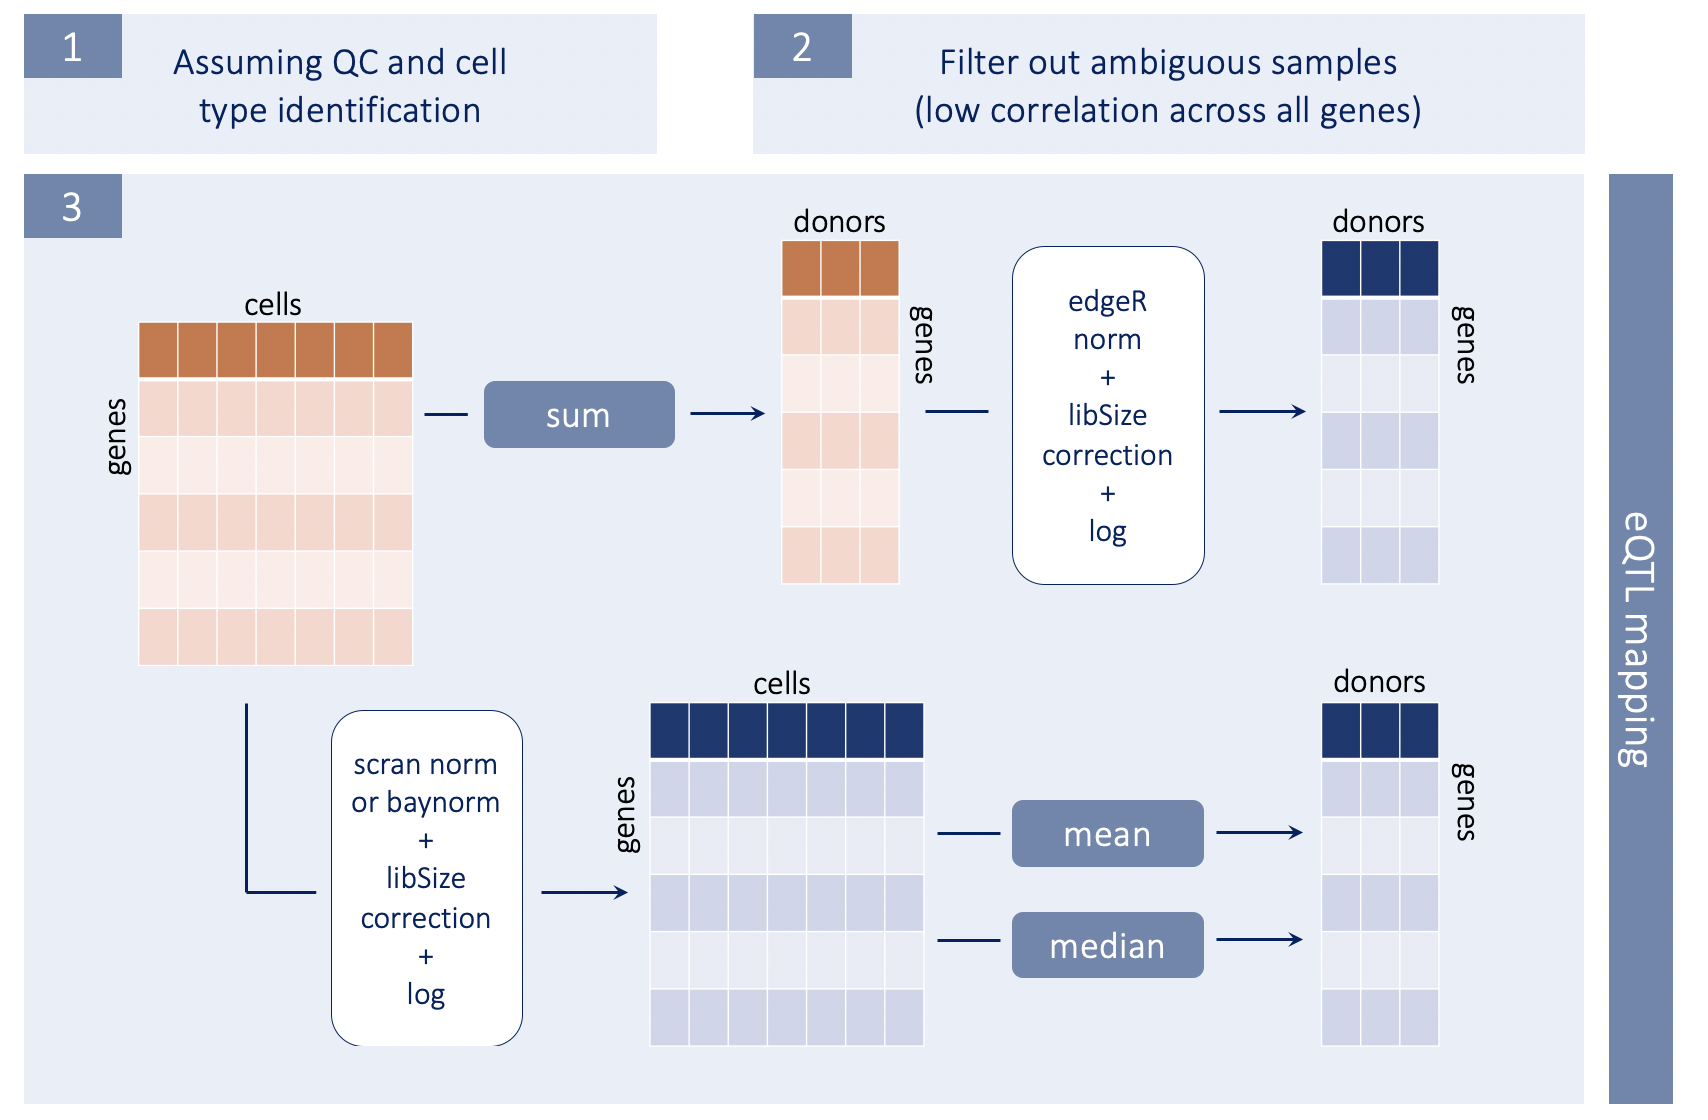
\includegraphics[width=15cm]{Chapter3/Fig/sc_qtl_workflow.png}
% \caption[sc-eQTL workflow]{\textbf{sc-eQTL workflow}.\\
% Placeholder: different approaches tested to perform \gls{eqtl} mapping using scRNA-seq profiles}
% \label{fig:sc_qtl_workflow}
% \end{figure}

% % \newpage

% \subsection{Covariates}

% % Expression covariates PCs, PEER established (add references, e.g. GTEx..)

% Another parameter we varied was the type and number of expression covariates included in the model to account for global expression variation (see section 2.2.3).

% In particular, we computed principal components (PCs) from the (aggregated) expression matrix.
% We also computed 10 MOFA factors \cite{argelaguet2018multi} as well as XX PEER factors \cite{stegle2010bayesian,stegle2012using}.

% Since the (total?) mean performed best as an aggregation method, we tested various number of covariates for this model only.

% In particular, we included 5, 10, 20 and 50 PCs in the model as covariates and evaluated performance.

% % % \section{Results in iPSCs}
% % \section{Results}




% % % \section{Results in simulated data}

% \clearpage

\section{Discussion}

% add little intro

% change below, from endodiff paper
The results presented in this chapter illustrate a difference between bulk and single-cell transcriptomics, as applied to eQTL mapping: the trade-off between statistical power and cellular resolution. 
Indeed, in this analysis of iPS cells, bulk transcriptomes provided higher statistical power for discovery of eQTL. 

However, iPSCs are very homogeneous...
In complex tissues such as brain, ..
% However, as we have demonstrated, a single-cell approach allows detailed annotation of changing eQTL effects across heterogeneous cell types and cell states, with the ability to better interpret the context-specific role of individual genetic variants. 
% As single-cell approaches are extended to more disease-relevant tissues and cell types, this may provide important clues on the causal role of genetic variants in disease. 
% The single-cell technology employed also has implications for what can be assessed. 

Pooling (vs bulk)

% ASE (vs 10x)

While we found that similar eQTL signals could be detected with both Smart-seq2 and 10x approaches, the full-length transcripts of Smart-seq2 allowed quantification of ASE, which is not possible with the 3' fragments sequenced using the 10x protocol.
A further advantage of the application of single-cell transcriptomics in this study was to enable the pooling strategy. 
While the feasibility of pooling samples has previously been demonstrated for peripheral blood mononuclear cells\cite{kang2018multiplexed}, we have extended this to cell lines differentiated together in culture. \\


% Is it relevant to do? 
% vs gating+bulk


% Comparison with bulk

% trade off: power vs resolution
% also pooling allowed using single cells

% Comparison across technologies

% plate-based vs droplet-based

